%!TEX encoding = IsoLatin

\documentclass[12pt]{ULrapport}
\usepackage[ansinew]{inputenc}
\usepackage[french]{babel}
\usepackage{float}
\restylefloat{table}
\usepackage{hhline}
\usepackage{pdfpages}
\usepackage{hyperref}
\usepackage{multirow}


% Title Page
\title{Design III: Pirates des Cara�bes}
\author{S�bastien Garvin, Xavier Kedzierski, Matthieu Sylvain, J�r�my Brown, Charles-Olivier Magnan, Jean-Michel Provencher}



\TitreProjet{Design III}                       
\TitreRapport{Remise 2}                      
\Destinataire{Philippe Gigu�re, Dominique Grenier, Denis Laurendeau}         
\NumeroEquipe{7}                                     
\NomEquipe{Zi�re}                               
\TableauMembres{%
	111\,114\,478  & Garvin, S�bastien   & \\\hline 
	111\,040\,128  & Kedzierski, Xavier   & \\\hline     
	111\,066\,466  & Magnan, Charles-Olivier      & \\\hline
	111\,071\,384  & Provencher, Jean-Michel   & \\\hline     
	111\,073\,630	 & Bourque, Emile						& \\\hline
	111\,075\,478	 & Sylvain, Matthieu			& \\\hline
	111\,074\,361  & Brown, J�r�my				& \\\hline
	907\,196\,009  & Garneau, Laurent			& \\\hline
}
\DateRemise{28 f�vrier 2016} 
% Contenu de l'historique des versions
\HistoriqueVersions{%										% version & date & description \\\hline
       1.0  & 24 janvier 2016 & Cr�ation du document \\\hline
			 2.0  & 31 janvier 2016 & Remise 1 \\\hline
			 3.0  & 28 f�vrier 2016 & Remise 2 \\\hline
			}

\begin{document}

% Chapitres
\chapter{Diagrammes}
\label{s:Diagrammes}


\section{Diagramme de contexte}
\label{s:Diagramme_contexte}

\begin{figure}[htp]
   \centering
   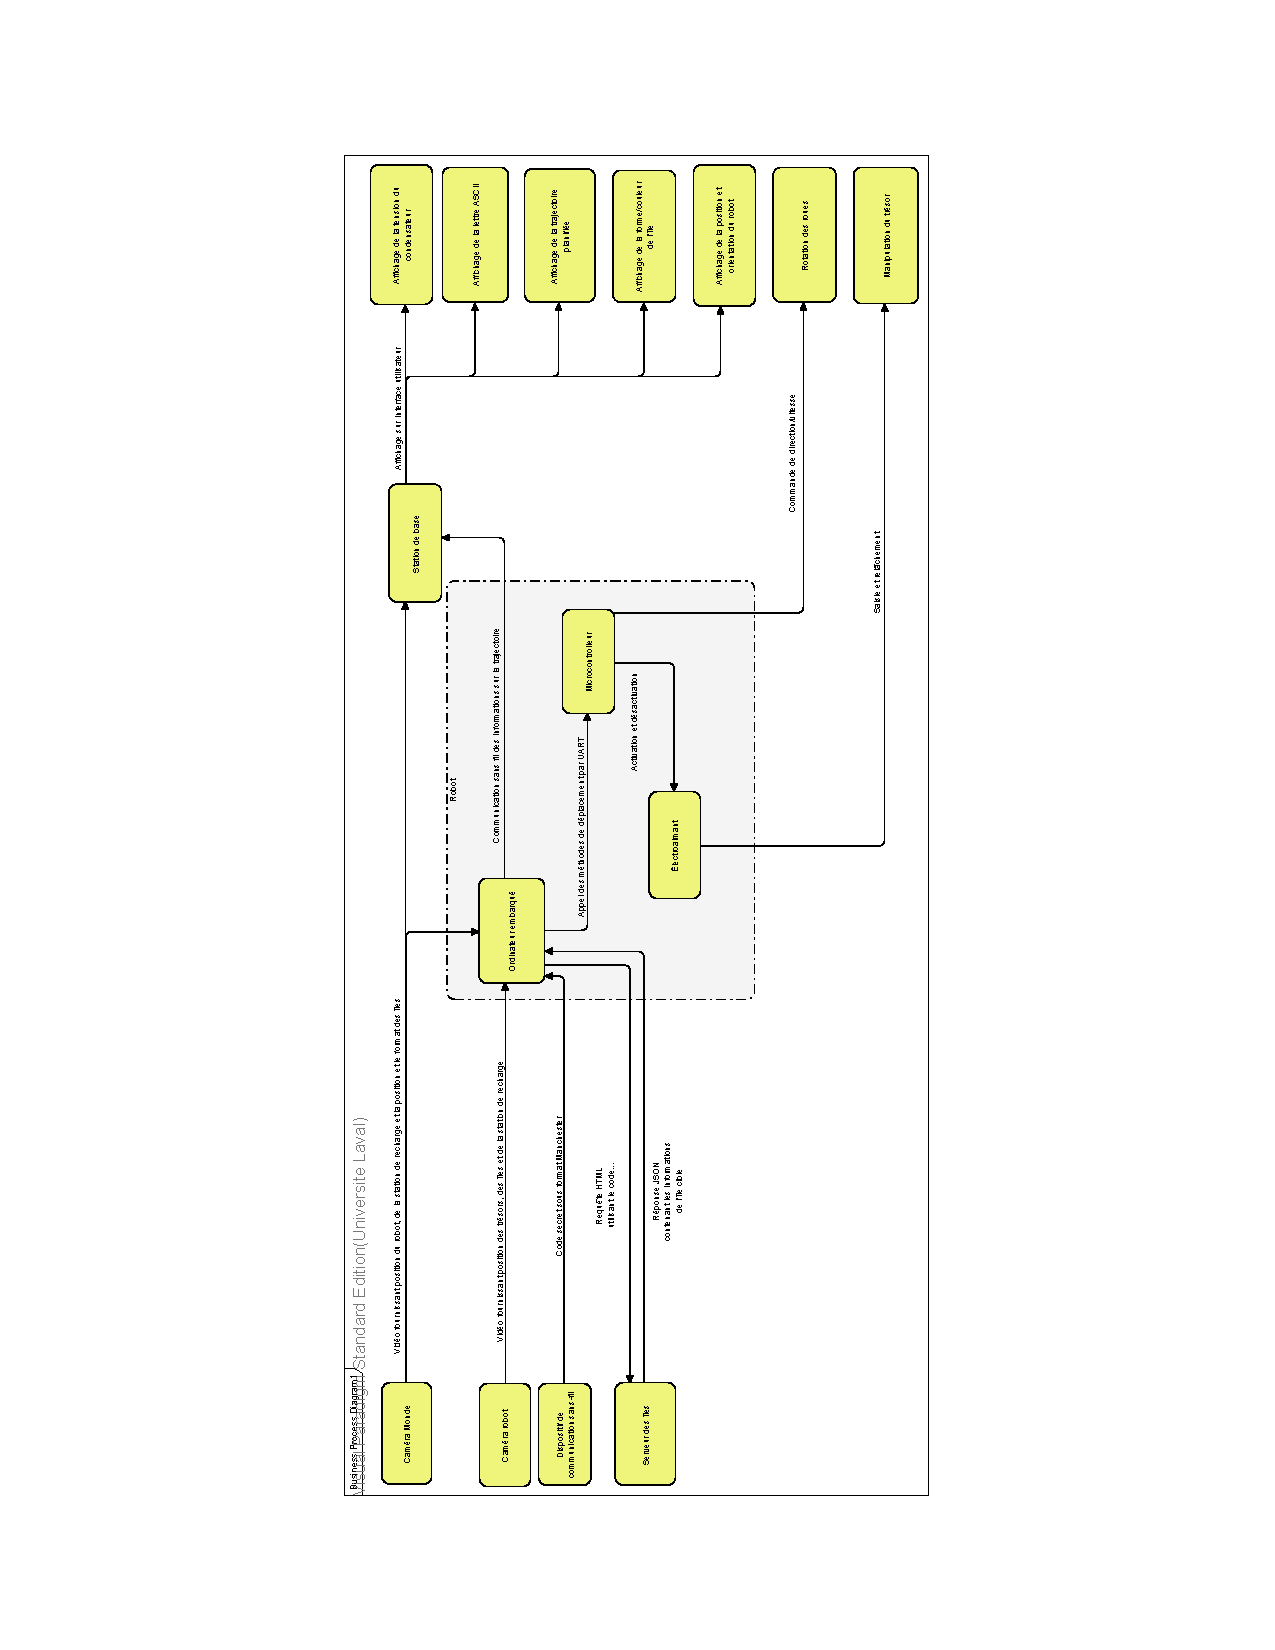
\includegraphics[width=0.75\textwidth, angle =-90]{pdf/ContextDiagram.pdf}
   \caption{Diagramme de contexte}
   \label{f:Diagramme_contexte}
\end{figure}

\newpage

\section{Diagramme de classes}
\label{s:Diagramme_classes}

\begin{figure}[htp]
   \centering
   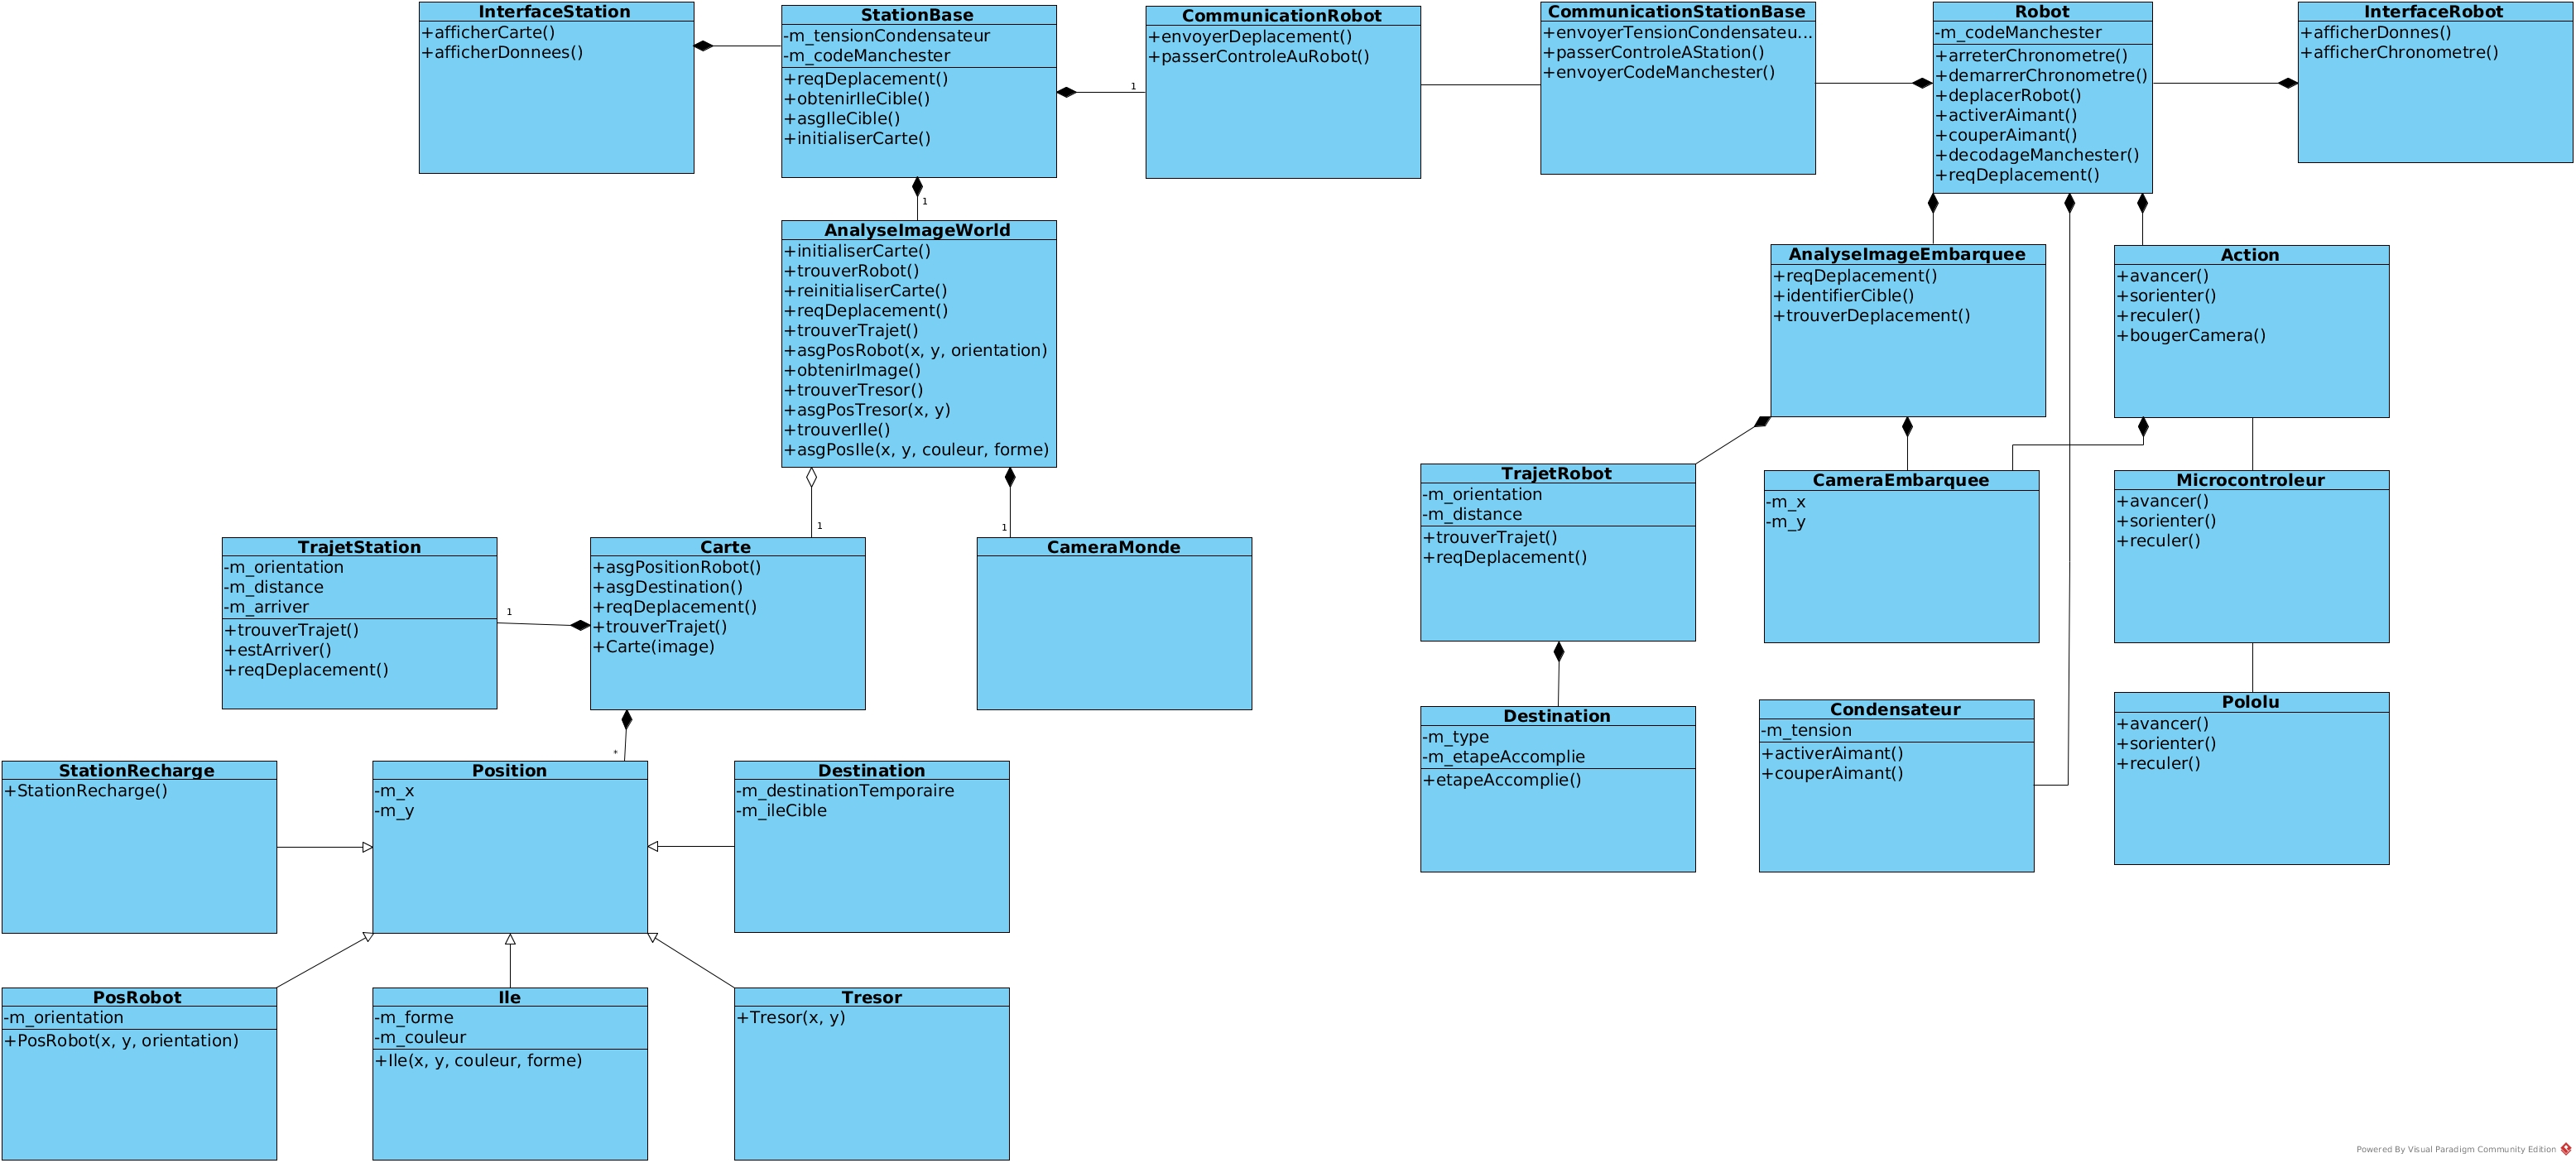
\includegraphics[width=0.95\textwidth, angle =-90]{fig/ClassDiagram.jpg}
   \caption{Diagramme de classes}
   \label{f:Diagramme_Classes}
\end{figure}

\newpage


La figure \ref{f:Diagramme_Classes} repr�sente le diagramme de classes suite � la premi�re it�ration. La structure est suseptible de changer suite aux prochaine it�rations, mais voici une br�ve description de la structure sur laquelle nous nous entendons pr�sentement. \par

La section de gauche du diagramme sera impl�ment�e sur la station de base tandis que la section droite sera impl�ment�e sur le robot. Ces deux syst�me pouront communiquer entre eux � l'aide des classes CommunicationRobot et CommunicationStationBase. \par

En ce qui conscerne la station de base, le contr�leur du syst�me est repr�sent� par la classe StationBase. La classe AnalyseImageWorld analyse les images re�u de la CameraMonde et g�n�re une carte sh�matique de la table (Carte) � l'aide d'imagerie. La carte est compos�e de diverses �l�ments qui h�rite tous de la classe Position. Les trajectoires du robot seront calcul� dans la classe TrajetStation � l'aide des informations de la classe Carte.  \par

Pour ce qui est du robot, il est aussi compos� d'un contr�leur (Robot). Les mouvements que devra effectuer le robot passerons tous par la classe Action qui les acheminera au microcontroleur et au polulu si nescessaire. Lorsque le robot est pr�s de la destination, TrajetRobot calculera les trajets (� l'aide de Destination et d'imagerie effectu� dans AnalyseImageEmbarquer).

    
   



\section{Diagramme de s�quences}
\label{s:Diagramme_sequences}

\begin{figure}[htp]
	\centering
	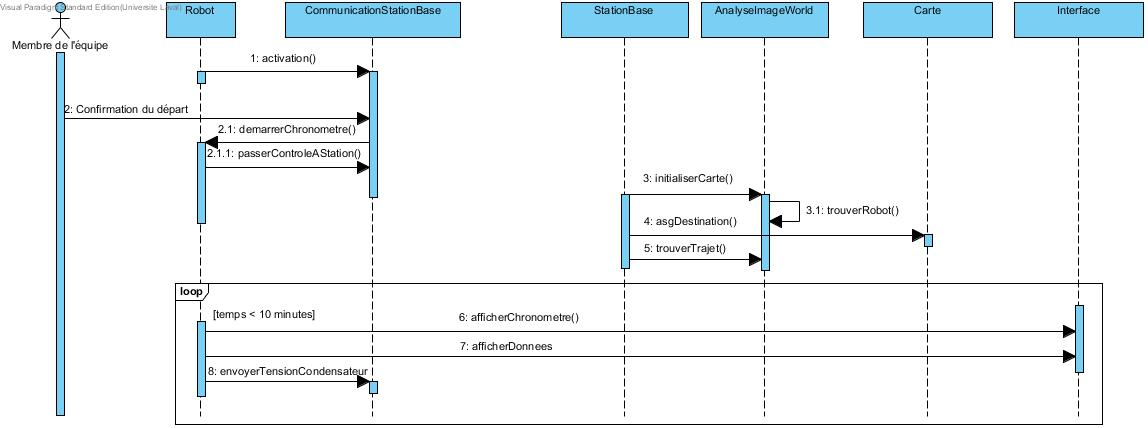
\includegraphics[width=0.95\textwidth]{fig/demarrageRobot.jpg}
	\caption{D�marrage du Robot}
	\label{f:DemRob}
\end{figure}

%\begin{figure}[htp]
%   \centering
%   \includegraphics[width=1\textwidth]{Diagramme_sequences}
%   \caption{Diagramme de s�quences}
%   \label{f:Diagramme_sequences}
%\end{figure}


\chapter{Plan d'int�gration}
\label{s:PlanIntegration}


\begin{figure}[htp]
   \centering
   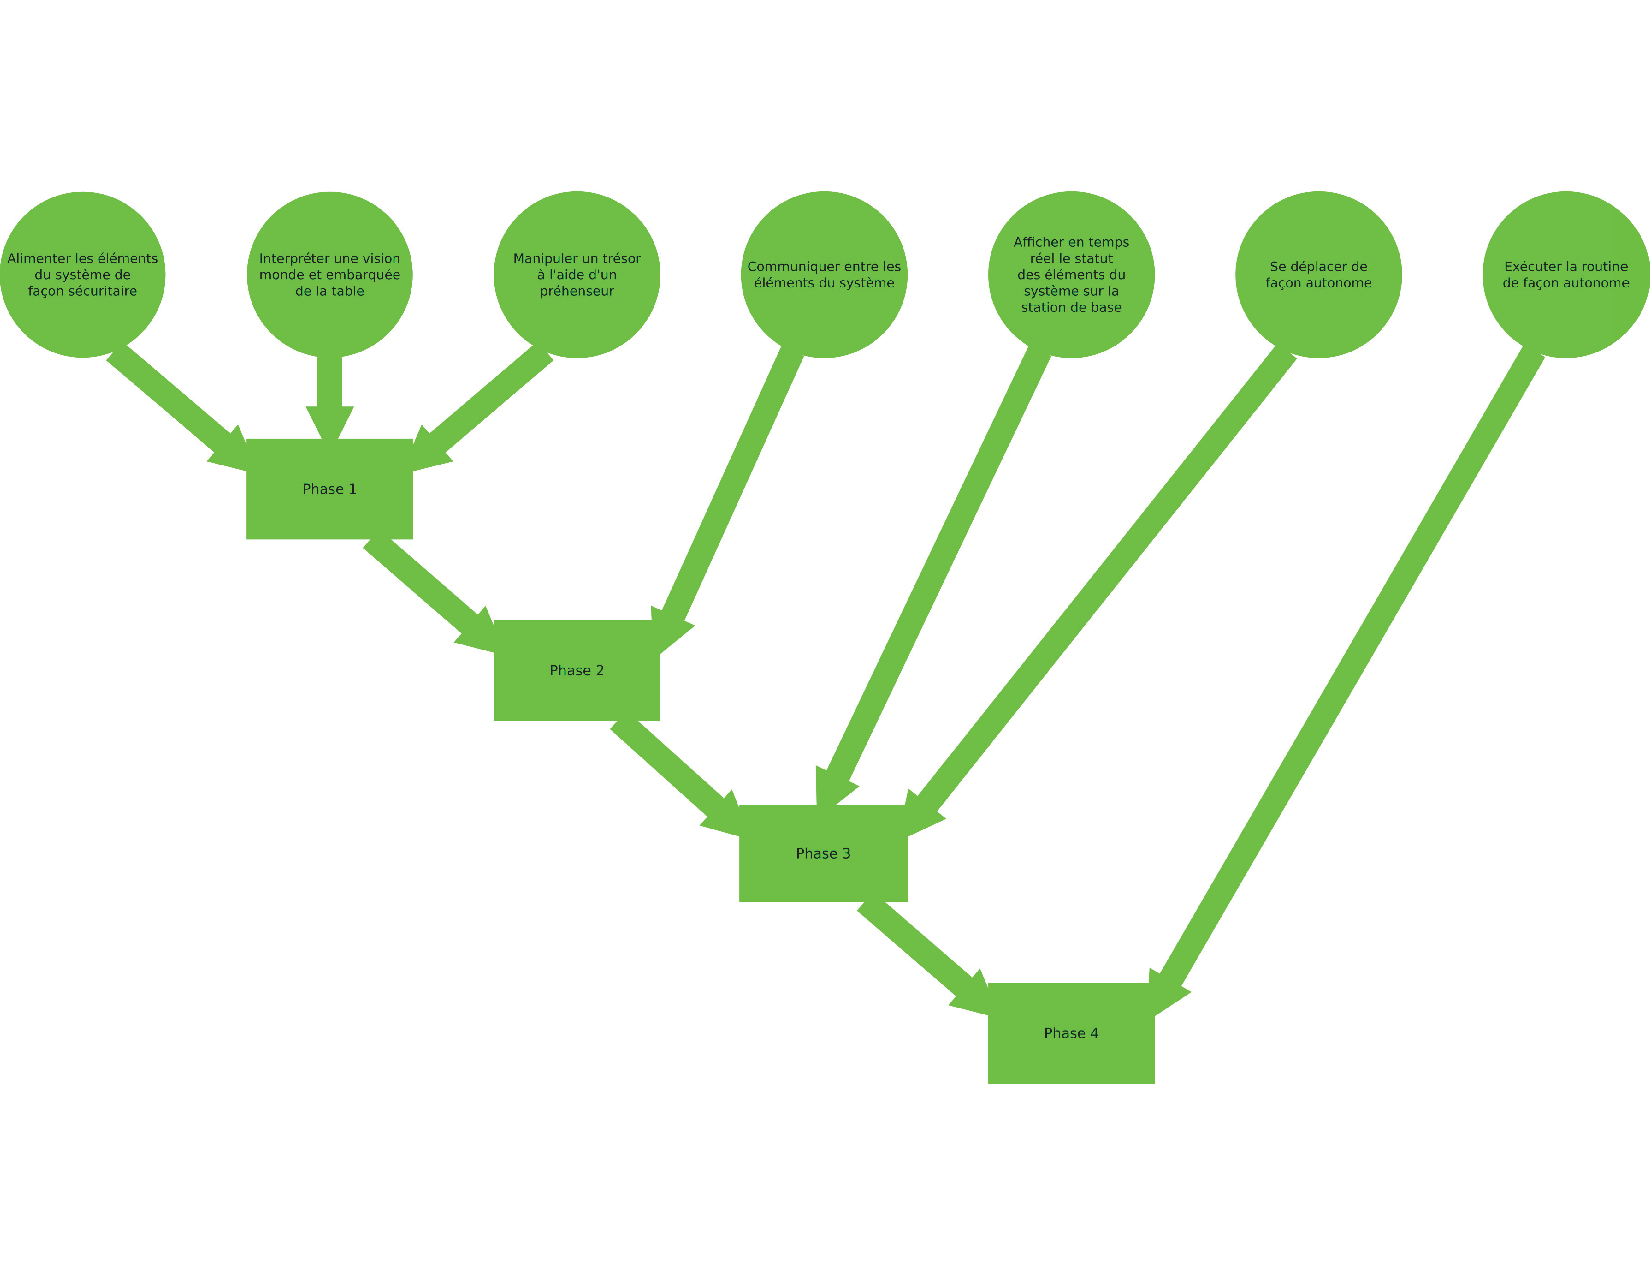
\includegraphics[width=1\textwidth]{pdf/PlanIntegration.pdf}
   \caption{Plan d'int�gration}
   \label{f:plan_integration}
\end{figure}



\chapter{Avancement de la construction du syst�me}
\label{s:AvancementConstruction}



\section{Structure m�canique}
\label{s:structure_mecanique}

L'un des points important de l'aspect physique du robot est d'avoir un centre de gravit� assez bas pour �viter � celui-ci de basculer en cas de d�part brusque. Un poids assez important pour coller le robot au sol est aussi important pour ce point. Pour atteindre cet objectif il serait id�al de placer l'ordinateur embarqu� sur l'�tage inf�rieur puisqu'il est le syst�me le plus lourd. Il fut cependant d�cid� de le placer sur l'�tage au-dessus afin de lib�rer cet �tage pour placer l'�lectronique et la batterie, r�duisant ainsi la longueur des fils n�cessaires pour se rendre aux moteurs par exemple.
\medbreak
Un autre point important est d'assurer un support solide aux circuits �lectroniques ainsi qu'� la batterie. � cet effet une feuille de contreplaqu� est install�e sur l'�tage inf�rieur afin de visser les circuits sur celle-ci. Bien �videmment des trous pour des vis sont int�gr�s aux circuits et la feuille elle-m�me est fix�e � la base du robot. L'interrupteur principal de l'alimentation est mont� sur le c�t� du robot de fa�on � �tre accessible facilement. Les fusibles sont dispos�s pour pouvoir �tre chang�s facilement en cas de besoin. On minimise ainsi l'espace perdu sur le robot. 

\section{Communications sans fil}
\label{s:communications_sans_fil}

Afin de pouvoir communiquer entre le robot et la station de base, une communication sans-fil est nécessaire. Comme il est important d’établir une connexion avec détection perte de paquet, le protocole TCP a été choisi. Grâce à ce protocole, on s’assure que les paquets perdus seront retransmis afin de ne perdre aucune information dans la communication sans-fil entre le robot et la station de base. Ainsi, en agissant comme serveur, la station de base attendra une connexion client de la part du robot. Une fois cette connexion établie, un échange de fichier JSON contenant des commandes et des paramètres pour le robot s’effectuera. Les avantages d’utiliser un format de fichier JSON pour l’échange est qu’il est simple à implémenter dans plusieurs langages et qu’il est plus facile à parser que le XML.

\section{Alimentation}
\label{s:alimentation}

Pour alimenter ad�quatement tous les syst�mes pr�sents sur le robot, on doit avoir une batterie avec un voltage qui se situe entre 21V et 30V pour alimenter le r�gulateur de l'ordinateur embarqu�, qui fonctionne � 19V avec un courant de 3.5A. On doit �galement avoir assez de puissance pour que les moteurs et l'�lectronique de contr�le puissent fonctionner pendant au moins dix minutes. La puissance dont le robot a besoin se d�finit surtout par celle des moteurs, des servomoteurs et de l'ordinateur embarqu�. Les moteurs demandent au maximum 800mA � 12V lorsque le rotor est compl�tement bloqu� et les servomoteurs qui servent � contr�ler la cam�ra demandent environ 30mA � 5V lorsqu'ils sont sollicit�s, soit un court instant. On utilise �galement un servomoteur plus puissant pour d�placer le pr�henseur, celui-ci risque de consommer plus de puissance � cause de l'effort plus important qui sera fourni. En additionnant la puissance de ces syst�mes, la puissance requise est d'environ 110W dans le pire des cas. Nous avons donc choisi une batterie LiPO 6S de 4 500mA, ce qui peut donner 27A, pour un total de 599W en 10 minutes. Les six cellules sont n�cessaires pour avoir 22.2V, ce qui permet d'obtenir le 19V requis pour l'ordinateur embarqu�. Le 4 500mA est justifi�, car on veut pouvoir travailler sur le robot plus longtemps que 10 minutes � des fins de test. Nous avons calcul� que cette batterie pourrait nous donner environ 50 minutes d'autonomie. 
\bigbreak
L'utilisation d'une batterie LiPO n�cessite un chargeur intelligent qui refuse de charger la batterie si les cellules ont un voltage trop faible, car la batterie pourrait exploser. Nous avons donc achet� un tel chargeur et on utilise �galement un sac de protection pour diminuer l'impact d'une �ventuelle explosion. L'utilisation d'une LiPO requi�re �galement un syst�me qui d�clenche une alarme sonore lorsqu'il faut recharger la batterie, pour justement emp�cher les risques d'explosions. Cette fonction est assur�e par un petit afficheur de tension, con�u sp�cialement pour les batteries LiPO, qui sonne quand la tension des cellules est trop faible. 
\bigbreak
Le robot a donc besoin de trois niveaux de tension diff�rents pour fonctionner. On utilise des r�gulateurs DC-DC pour avoir une tension stable, aux tensions d�sir�es. Le r�gulateur de l'ordinateur embarqu� est fourni. Pour le 12V et le 5V, nous avons choisi de prendre trois fois le m�me r�gulateur, qui prend 4V � 38V en entr�e et peut fournir 1.25V � 36V en sortie. Il y aura donc deux r�gulateur pour le 12V, pour s�parer l'alimentation des moteurs et celle du Arduino, et un r�gulateur pour le 5V. Ce r�gulateur peut fournir un maximum 5A et il est dot� d'un afficheur de tension pour conna�tre facilement le niveau de tension en sortie. On prot�ge nos syst�mes avec des fusibles pour s'assurer de ne rien briser. On a choisi de prendre un fusible de 10A directement � la sortie de la batterie pour prot�ger l'ensemble du syst�me. Pour les moteurs, on utilise un fusible de 5V, ensuite un fusible de 2A pour l'alimentation de l'Arduino et enfin un fusible de 3A pour les circuits �lectroniques du 5V. Un interrupteur situ� directement suite � la batterie permet finalement d'actionner l'ensemble du syst�me. La figure \ref{f:alim} pr�sente un diagramme en bloc de l'alimentation.

\begin{figure}[htp]
   \centering
   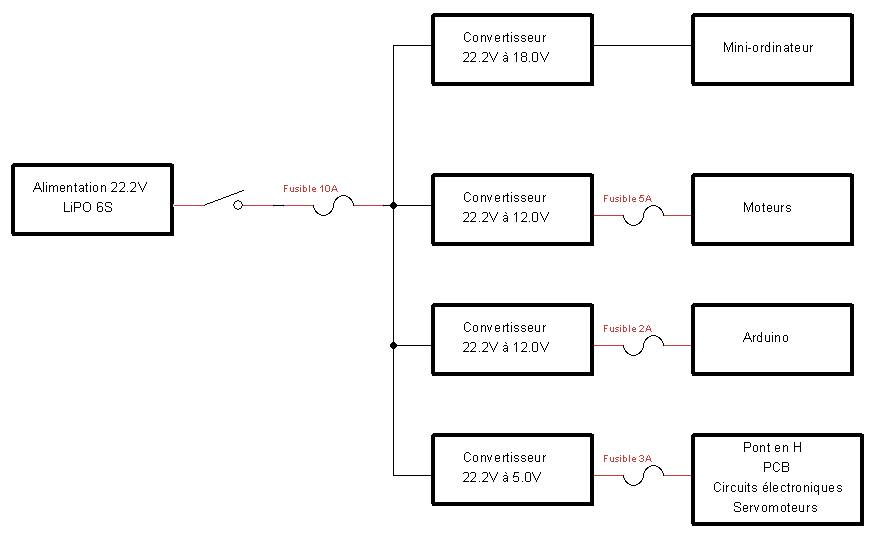
\includegraphics[width=1\textwidth]{fig/alim.jpg}
   \caption{Diagramme en bloc de l'alimentation}
   \label{f:alim}
\end{figure}


\section{Contr�le et asservissement des moteurs}
\label{s:controle_asservissement}

Afin de contr�ller les roues, la premi�re �tape est d'alimenter correctement chacun des moteurs des roues. Le pont en H connect� aux moteurs n�cessite trois entr�es par roue: deux entr�es servent � s�lectionner la direction des roues, et une troisi�me re�oit un PWM d�terminant la vitesse de rotation de la roue.

Le pont en H est aliment� � l'aide d'une alimentation 5V, ce qui pour les fins de la d�monstration est fait directement � partir d'une sortie de l'Arduino Mega. Les encodeurs des roues en tant que tels sont par contre doivent �tre aliment�s � une tension entre 3.5 et 20V, temporairement fourni � l'aide d'une source murale. Selon les sp�cifications du pont en H, la pin 1 de chaque moteur doit re�evoir une tension faible et la pin 2 une tension �lev�e pour tourner la roue associ�e dans le sens des aiguilles d'une montre. Afin de tourner dans le sens inverse, il faut alors utiliser une tension �lev�e sur 1 et faible sur 2. Un des premiers tests est alors effectu�, avec le pont en H aliment� et les quatres roues � pleine vitesse. � l'aide de ce test, il fut facile de voir que le branchement des roues de m�me orientation devrait �tre de deux sens oppos�s, car le sens des aiguilles signifie une rotation diff�rente d'un c�t� � l'autre du robot.

Par la suite, en utilisant des sorties PWM de l'Arduino Mega, des ondes carr�es � rapport cyclique de 50\% sont envoy�es en sortie. Celles-ci, lorsque connect�es aux entr�es de vitesse correspondant aux quatres moteurs dans le pont en H, permettent de comparer la vitesse des moteurs et de v�rifier si celle-ci est consistente. R�sultat de ce test: en activant deux roues � la fois, le robot ne va pas en ligne droite. Le moteur 1 fait tourner la roue significativement plus rapidement que le moteur 3 avec la m�me commande. Un asservissement avec int�grateur est donc absolument n�cessaire afin que la vitesse de chaque roue rejoigne la consigne, permettant au robot de rouler en ligne droite.

La librarie PID disponible sur le Playground Arduino permet de rapidement impl�menter un asservissement avec une dur�e d'�chantillonage, une commande � rejoindre et des param�tres kp, ki et kd d�finis par l'utilisateur. Pour impl�menter la commande � rejoindre, les encodeurs des moteurs sont branch�s directement � des entr�es num�riques du microcontr�lleur Arduino. En effet, ceux-ci g�n�rent une onde carr�e � largeur variable, celle-ci pouvant �tre lue en utilisant la fonction pulseIn(). La dur�e de lecture maximale (timeout) de la largeur d'impulsion est � la base tr�s lente, environ une seconde par lecture, ce qui rend l'asservissement peu efficace si le robot tourne lentement. Pour rem�dier � cette situation, un timeout de 3 ms a �t� choisi.

Avec pulseIn, lorsqu'aucune onde n'est d�tect�e avant la fin du temps maximal, une valeur de 0 est retourn�e. Hors, l'asservissement fonctionne avec un principe que lorsque la dur�e retourn�e par pulseIn est sup�rieure � la commande, il faut augmenter la sortie vers les moteurs. Afin d'assurer qu'une roue � l'arr�t ne soit pas consid�r�e comme impossiblement rapide, une valeur de 0 est remplac�e par la dur�e maximale de lecture, soit 3 ms.

Les tests initiaux de l'asservissement �taient peu fructueux. En effet, la sortie du PID variait beaucoup trop rapidement entre minimum et maximum, ne permettant que tr�s peu de pr�cision. Ceci �tait d� � un kp trop �lev�, ce qui multipliait l'erreur bien au del� de la valeur maximale du param�tre du PWM, soit 255. En diminuant l'�l�ment proportionnel kp � 0.0005 au lieu de 1, la variation cyclique due � un trop large d�passement est �vit�e. Le ki est pr�sentement � 0.25 car il permet de rejoindre la consigne suffisemment rapidement sans cr�er de trop larges d�passements.

\begin{figure}[htp]
	\centering
	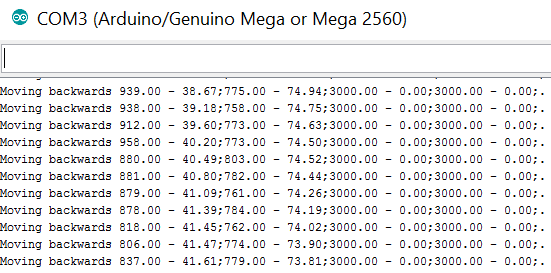
\includegraphics[width=1\textwidth]{fig/communicationArduino.png}
	\caption{Test de rotation sur deux roues, commande � rejoindre de 800 microsecondes de largeur d'impulsion}
	\label{f:test_Arduino}
\end{figure}

Dans l'�tat actuel de ce sous-syst�me, il y a d�passement en vitesse de plus de 10\% pendant environ une seconde. Afin de permettre des d�plaements plus pr�cis, du travail sera fait pour diminuer ce d�passement. Pour communiquer � l'Arduino Mega la ccomnsigne � rejoindre, une interruption sur le port s�rie est impl�ment�e en utilisant serialEvent. Lorsque le port s�rie d�tecte qu'il y a quelque chose � lire sur le port s�rie, le code de lecture de la commande prend alors priorit� sur l'ex�cution du PID.

\section{Pr�henseur et �lectroaimant}
\label{s:prehenseur_electroaimant}

Afin de conserver l��nergie dans le condensateur le plus longtemps possible, le courant de d�charge dans l��lectroaimant est limit� par un MOSFET. Une onde carr� de largeur d�impulsion variable est envoy�e dans sa base et permet de contr�ler ce courant. 
\medbreak
Avec un condensateur de 5F charg� � 5V et du limiteur de courant, l'�lectroaimant peut soulever un tr�sor durant 3 � minutes, ce qui est largement suffisant pour le projet.
\medbreak
Le syst�me comprend aussi un interrupteur �lectronique afin de permettre de couper la d�charge de courant dans l��lectroaimant et ainsi d�poser le tr�sor.


\section{Code Manchester}
\label{s:Manchester}

Le syst�me de transmission retenu par l'�quipe pour communiquer le signal Manchester est un syst�me utilisant une LED comme �metteur et une autre LED comme r�cepteur. Ce syst�me LED � LED est une solution simple et peu co�teuse qui ne pr�sente donc pas un co�t mon�taire important pour le projet ni beaucoup de temps de travail. Pour d�coder le code il est n�cessaire de transmettre l'horloge ainsi que le code, le syst�me est donc install� en double � cet effet. Chacun des signaux est transmis par un banque de quatre LED qui seront situ�es sur la station de recharge. L'utilisation de plusieurs diodes est justifi�e pour rendre le syst�me plus efficace en cas de d�faillance d'une de celle-ci et donc d'ajouter de la redondance. Les LED en r�ception sont situ�es de chaque c�t� de la face avant du robot de mani�re � �viter les interf�rences. Encore une fois, la redondance est utilis�e pour la r�ception et deux LED sont donc plac�es � cet effet.
\medbreak
L'horloge fournit avec le dispositif du Manchester n'est pas utilis�e car elle est jug�e trop rapide, une horloge d'environ 1 � 2Hz est g�n�r� par un microcontr�leur PIC. Une fr�quence plus �lev�e n'est pas requise d� au temps pass� � recharger le condensateur, de plus, avec une basse fr�quence le risque d'erreur est jug� moins �lev�. Des LED rouges sont utilis�es pour la transmission des signaux, apr�s des exp�riences avec d'autres couleurs il fut remarqu� que celles-ci offraient les meilleures performances.
\medbreak
Un circuit d'amplification des signaux situ� sur le robot permet d'amplifier ceux-ci apr�s r�ception et donc de produire des signaux 0 � 5V. Le sch�ma de ce circuit est pr�sent� � la figure \ref{f:Manchester} et r�alis� sur PCB conform�ment aux exigences. Les signaux amplifi�s sont ensuite lu par des entr�es num�riques de l'Arduino Mega. La signal d'horloge est lu par une entr�e permettant d'utiliser les interruptions tandis que le code Manchester est lu par une entr�e ordinaire. Une interruption est lanc�e sur chaque front montant d'horloge, les deux donn�es sont alors lues et on effectue une op�ration XOR sur les signaux afin d'obtenir le signal d�cod�. Ce r�sultat est ensuite stock� dans un buffer circulaire de 32 �l�ments, ce qui assure d'avoir au moins une it�ration de la s�quence de 16 bits dans son ensemble. Un algorithme parcours ensuite ce tableau de donn�es pour recherch� la s�quence de 8 bits � 1 suivit d'un bit � 0 pour finalement prendre les 7 bits d'int�r�t composant la lettre ASCII voulue. Cette lettre est finalement transmise � l'ordinateur embarqu�e pour utilisation future.

\begin{figure}[htp]
   \centering
   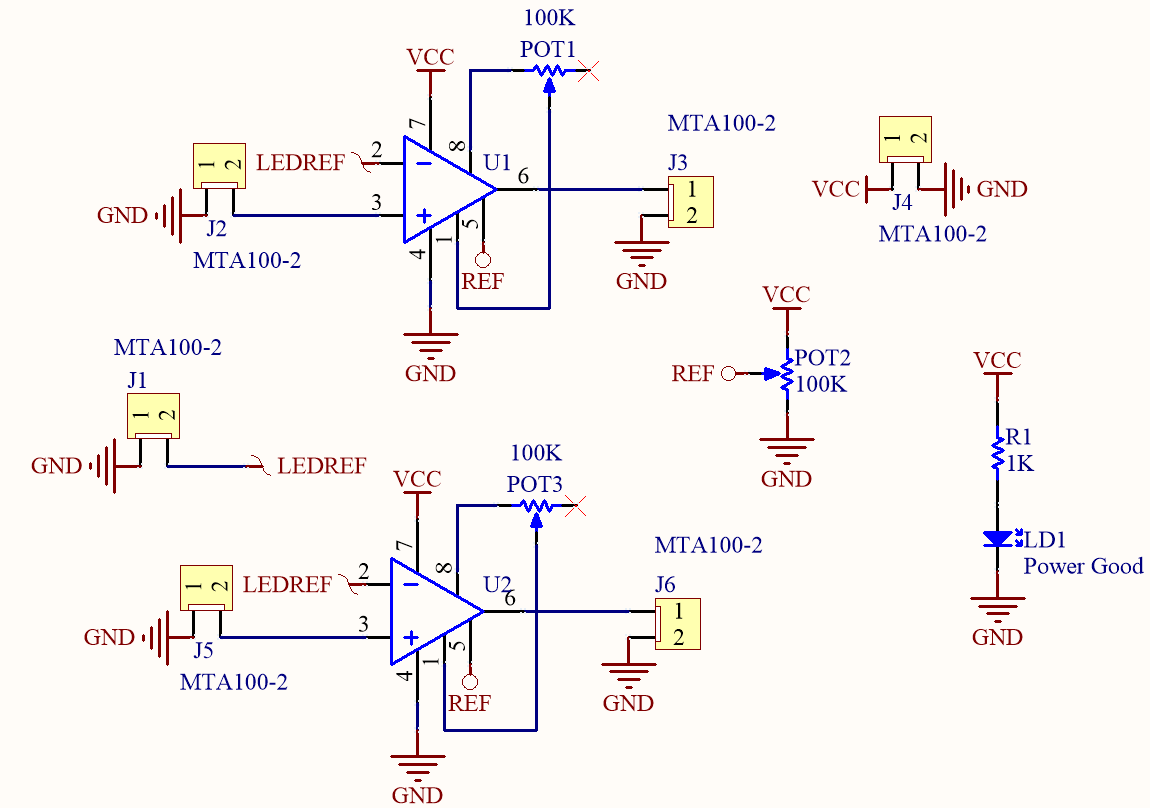
\includegraphics[width=0.85\textwidth]{fig/Manchester.png}
   \caption{Circuit d'amplification des signaux du code Manchester}
   \label{f:Manchester}
\end{figure}

\pagebreak

\section{Induction pour recharge}
\label{s:induction_recharge}

L��lectroaimant est aliment� par un condensateur. Ce dernier est recharg� par un transformateur. Le primaire du transformateur est situ� sur la station de recharge sur le bord de la table. Il est aliment� par la tension DC de 5V/3A qui provient de la carte Manchester. Le transformateur ne fonctionnant qu�en AC, il est n�cessaire de hacher cette tension DC. 
\medbreak
Plusieurs m�thodes existent pour hacher une tension DC. Nous avons choisi d�utiliser un simple MOSFET de puissance dans lequel nous commandons la base avec un horloge. Ce choix a �t� fait pour sa simplicit�. Il est en effet beaucoup plus simple � impl�menter qu'un pont en H. �galement, avec un seul MOSFET, nous limitions les pertes par dissipation dans les MOSFETs. L'horloge provient d'un microprocesseur situ� �galement sur la station de recharge. Diff�rentes fr�quences ont �t� test�es pour ce hacheur. Les fr�quences inaudibles (plus de 20kHz) sont plus int�ressantes, car notre oreille ne peut pas entendre ces fr�quences et le transformateur n'est donc pas bruyant. Toutefois, � ces fr�quences, l'effet inductif des bobines du transformateur devient tr�s grand et r�duit le courant qui traverse le transformateur. 
\medbreak
Comme un plus grand courant dans le transformateur �quivaut � une recharge plus rapide du condensateur, une fr�quence de 4kHz a �t� choisie. C'est � cette fr�quence que l'effet inductif des bobines du transformateur devient assez faible pour laisser passer un courant dans le transformateur assez grand pour avoir une recharge rapide du condensateur. De plus, si on descend � une fr�quence plus basse que 4kHz, l'effet inductif du transformateur devient tr�s faible; un courant trop �lev�e y circule et les deux bobines s'attirent fortement par aimantation. C'est pourquoi la fr�quence de 4kHz est choisie.
\medbreak
Toutefois, un condensateur ne peut �tre recharg� par une tension alternative. C'est pourquoi au secondaire se trouve un redresseur. Des tests ont �t� faits afin de choisir entre un redresseur simple alternance ou double alternance. Le redresseur double alternance a �t� choisi, parce qu'il est plus efficace.
\medbreak
Le condensateur choisi est un condensateur de 5F. Avec notre syst�me d'induction, il est possible de charger ce condensateur jusqu'� 5V. Des tests ont �t� faits avec ce condensateur et ont permis de d�terminer qu'� partir de sa pleine charge, il est capable d'alimenter notre �lectroaimant avec le courant n�cessaire pour tenir un tr�sor pendant 3 minutes 30 secondes, ce qui est amplement suffisant pour le projet.
\medbreak
Finalement, nous avons un interrupteur �lectronique pour ouvrir le circuit de recharge lorsque la recharge est compl�t�e; sans cela, un faible courant de fuite circule dans le pont redresseur et d�charge lentement le condensateur. La figure \ref{f:Borne} pr�sente le sch�ma �lectrique du syst�me implant� sur le robot.

\begin{figure}[htp]
   \centering
   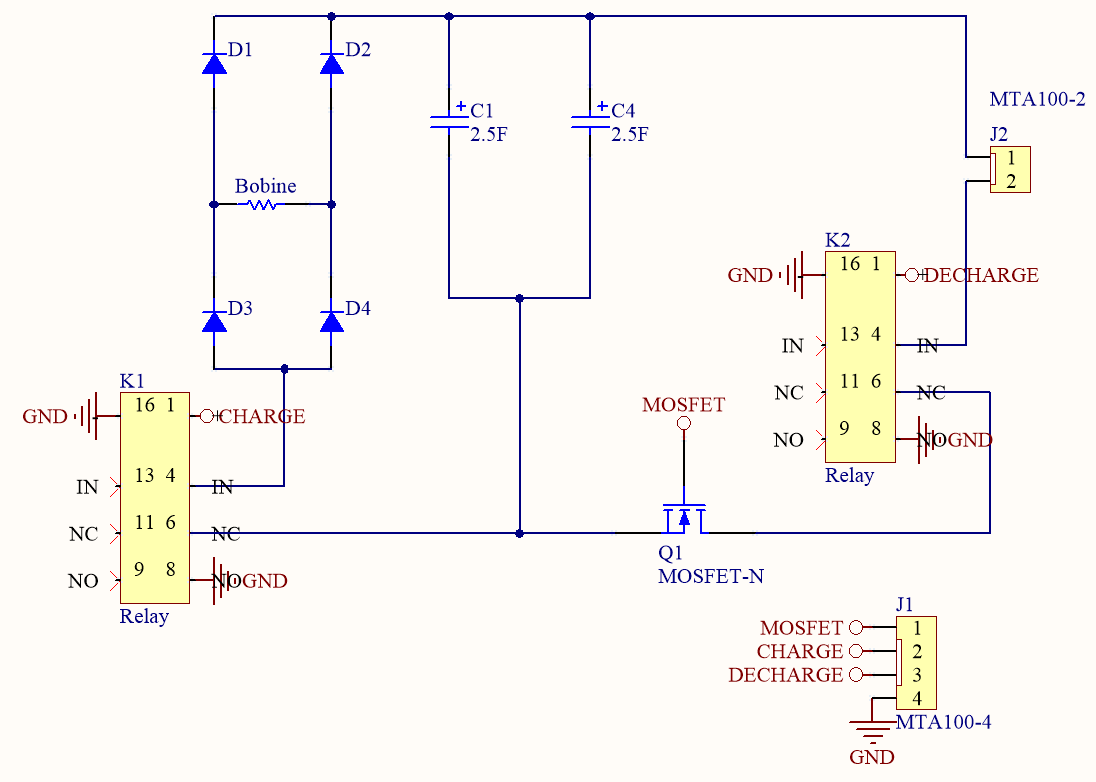
\includegraphics[width=0.85\textwidth]{fig/BorneChargement.png}
   \caption{Circuit de chargement et d�charge du condensateur}
   \label{f:Borne}
\end{figure}

\pagebreak

\section{Interface de la station de base}
\label{s:interface_station}


L'interface de la station de base est con�ue pour �tre simple comme le d�montre la figure \ref{f:InterfaceImage}. Elle a comme particularit� d'afficher une image virtuelle la plus semblable possible � l'image per�ue par la cam�ra monde.
\medbreak

\begin{figure}[htp]
   \centering
   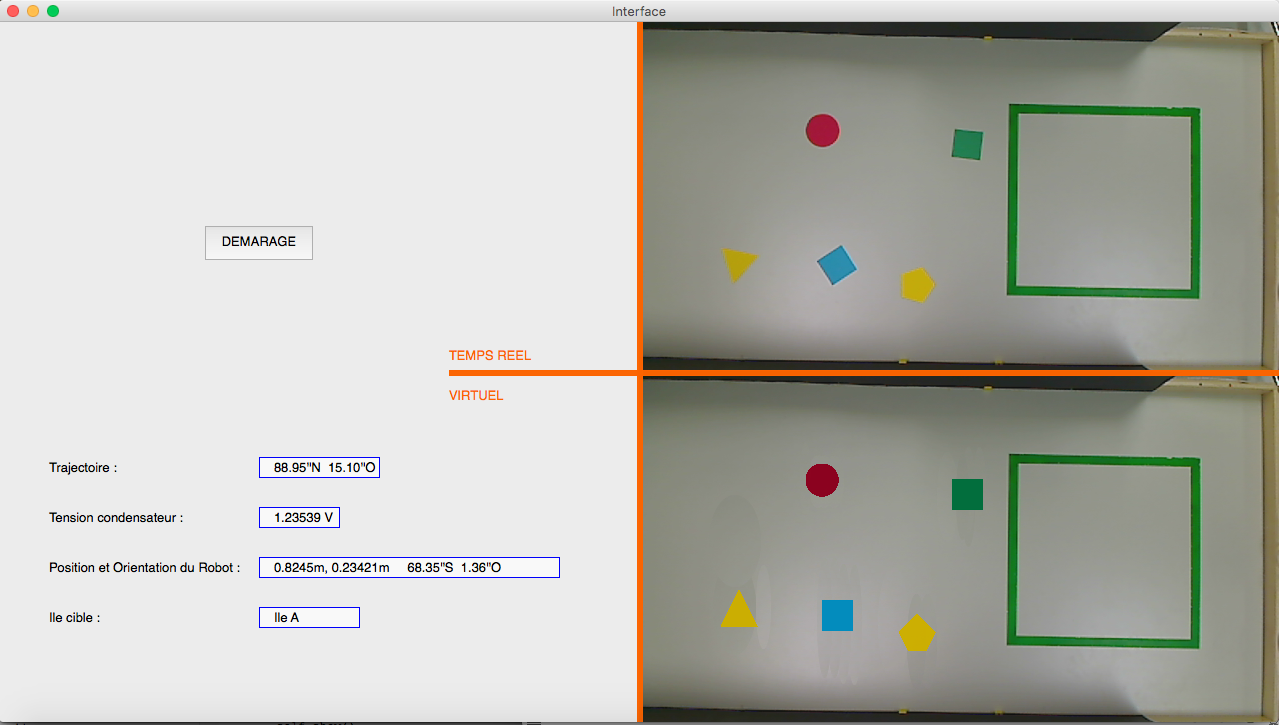
\includegraphics[width=1\textwidth]{fig/interface_Image.png}
   \caption{Interface de la station de base}
   \label{f:InterfaceImage}
\end{figure}

\medbreak
La section gauche de l'interface nous donne des informations sur la s�quence de jeu en g�n�ral. Elle affiche �galement des informations pertinentes sur le robot comme l'�le cible, l'orientation, la position et la direction du robot ainsi que la tension du condensateur.
\medbreak
Pour l'instant, l'interface n'est pas connect�e au syst�me, mais elle est plut�t pr�te � recevoir des informations telles que la position, la forme et la couleur d'un objet pour la reproduire de fa�on plut�t similaire dans l'image virtuelle comme le d�montre la partie inf�rieure droite de l'interface.
\medbreak
Le point fort de l'interface est l'id�e d'utiliser une photo de la cam�ra monde avant que les objets soient ins�r�s ou que le robot soit ins�r� pour ensuite ajouter des objets virtuellement. Ceci aide beaucoup plus � savoir si le syst�me saisi bien les formes, les emplacements et les couleurs de toutes sortes. On obtient une image semblable dans la section virtuelle en bas � droite de l'interface. On constate sur la figure que l'image en temps r�el est tr�s semblable � sa reproduction. La forme et la couleur sur le dessus du robot pour pouvoir bien d�terminer l'orientation et la position du robot n'ont toujours pas �t� d�termin�es. Par contre, lorsqu'elle sera d�termin�, il sera n�cessaire d'afficher le robot sur les cartes des images virtuelles et r�elles.
\medbreak
La trajectoire qu'emprunte le robot ainsi que la trajectoire planifi�e devront �tre int�gr� � cet environnement. Suite aux conseils re�us en cours, l'implantation d'options de d�marrage de tests � diff�rentes �tapes de la routine est pr�sentement explor�e.


\section{Planification de la trajectoire}
\label{s:planification_trajectoire}



La planification de la trajectoire est effectu�e avec les positions obtenues de la localisation (voir \ref{s:localisation}). Pour l'instant, elle se d�roule comme suit. Premi�rement, une grille de cellules est initialis�e avec les coordonn�es pixels de l'image o� chaque cellule repr�sente une coordonn�e cart�sienne (x,y). Lors de cette cr�ation, les pixels qui sont situ�es � un intervalle pr�s des centres des �les (en x et en y) sont d�clar�es comme �tant inaccessibles. Il y a donc une zone tampon en forme de carr� autour de chacune des �les. De plus, la cr�ation de la grille est cr��e avec une incr�mentation en x et en y de sorte � conserver seulement les coordonn�es pixels situ�es � plus ou moins un centim�tre de distance (sur la table). \medbreak

La raison d'avoir une zone tampon en forme de carr� au lieu d'un cercle est simplement puisque l'impl�mentation est grandement simplifi�e. Bien que ceci ne soit pas optimal, une trajectoire pourra tout de m�me �tre trouv�e d� au nombre r�duit d'�les sur la table.  \medbreak

Une fois cette grille initialis�e, il suffit de fournir une coordonn�e de d�part et d'arriver � l'algorithme de planification de trajectoire. Celui-ci est une impl�mentation de l'algorithme A* (figure \ref{f:Trajectoire}). La raison pour laquelle cet algorithme fut retenue est principalement pour sa rapidit� d�ex�cution. En effet, bien qu'il ne choisi pas le trajet le plus court, il le trouve tr�s rapidement. Cela est primordial puisque le trajet sera recalcul� de fa�on fr�quente afin de compenser pour les incertitudes et les erreurs d'approximation. L'autre candidat qui pourrait remplacer l'algorithme A* est l'algorithme de Dijkstra. Cela permettrait d'obtenir le trajet le plus court. Par contre, cela d�pendra de sa performance. Cette solution sera explor�e prochainement.  \medbreak   

\begin{figure}[htp]
   \centering
   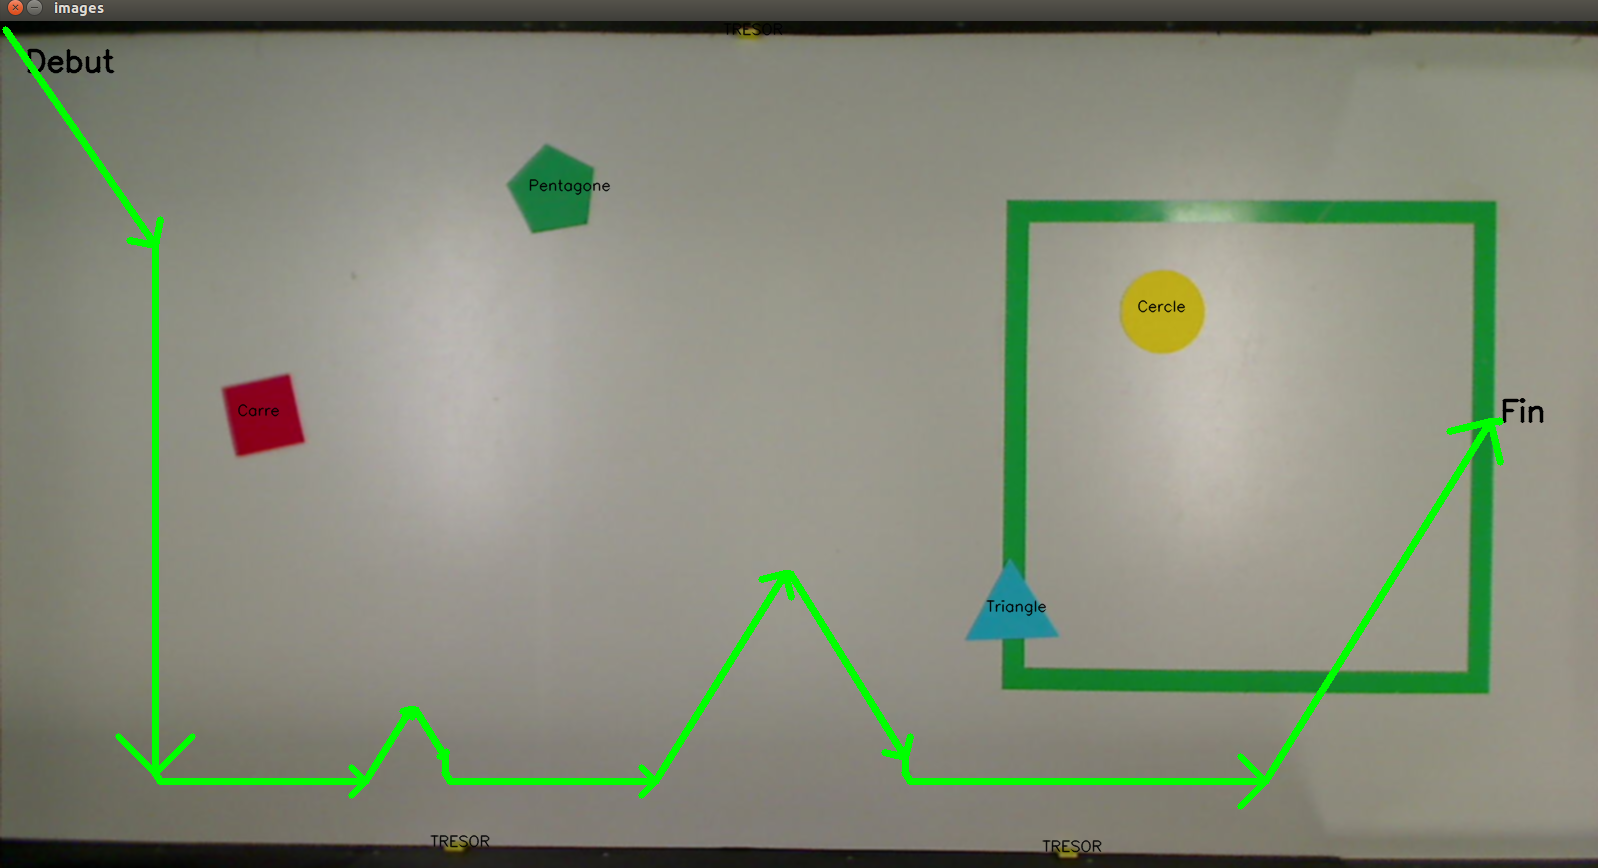
\includegraphics[width=1\textwidth]{fig/trajet.png}
   \caption{Exemple de trajectoire}
   \label{f:Trajectoire}
\end{figure}

En ce qui concerne la distance physique de plus ou moins un centim�tre des pixels dans la grille de cellules, il est sujet � changement. Pr�sentement, avec environ 3000 cellules dans la grille, l'algorithme A* s�ex�cute presque instantan�ment. Des tests seront effectu�es plus en profondeur selon l'algorithme choisi afin d'avoir une distance physique optimale entre les cellules.

       

\section{Contr�le de la cam�ra}
\label{s:controle_camera}

Le contrôle de la caméra embarquée s’effectue par des servomoteurs contrôlés par le Micro Maestro 6-Channel USB Servo Controller. Afin de simplifier les commandes nécessaires au contrôle de la position de la caméra, quatre positions prédéterminées ont été programmées : gauche, droite, avant, trésor. Comme ces quatre positions permettent de couvrir entièrement le champ de vision intéressant, il n’était pas nécessaire d’ajouter davantage de possibilités de contrôle de caméra. La position trésor correspond à la position avant dans laquelle la caméra regarde complètement vers le bas. Afin de déterminer ces positions, le logiciel Maestro Control Center a été utilisé pour noter les valeurs nominales de ces positions. Une fois les valeurs de position en main, une librairie Arduino a été développée afin de déplacer la position de la caméra dans ces différentes valeurs. Pour communiquer entre le Arduino Mega 2560 et le contrôleur de servomoteur

\section{Syst�me de vision}
\label{s:systeme_vision}

Les responsabilit�s du syst�me de vision sont partag�es entre la station de base et le robot. Le syst�me de vision sert � faire une analyse en profondeur de la table de jeu et � prendre des d�cisions gr�ce aux informations venant du robot. Le syst�me doit donc �tre performant et stable afin de ne pas induire le robot en erreur. 
\medbreak
La station de base, par l'entremise de la cam�ra monde, g�re la phase de d�placement tandis que le robot g�re la phase d'alignement � l'aide de sa cam�ra embarqu�e. La phase de d�placement comporte la d�tection des �l�ments cartographiques ainsi que la planification de la trajectoire alors que la phase d'alignement permet au robot de se positionner de mani�re optimale afin de faciliter l'ex�cution de la t�che demand�e.
\medbreak
La cam�ra monde est utilis�e pour la d�tection des �l�ments cartographiques ainsi que pour suivre le d�placement du tr�sor. Gr�ce � ces informations, la station de base peut g�n�rer une trajectoire et transmettre des commandes au robot.
\medbreak
La cam�ra embarqu�e ne sera utilis�e que dans deux situations. Tout d'abord, elle servira lorsque aucun tr�sor n'est d�tect� par la cam�ra monde, le robot tentera alors d'identifier la position des tr�sors gr�ce � son point de vue plus rapproch�. Ensuite, elle sera utilis�e lors de la phase d'alignement, afin que le robot puisse se rapprocher s�curitairement d'une cible comme une �le, un tr�sor ou la station de recharge. Donc, une fois la phase de d�placement termin�e et le robot rendu devant la cible, le syst�me de vision du robot prendra le contr�le afin d'amorcer la phase d'alignement.  



\section{Localisation des �les, des tr�sors et du robot}
\label{s:localisation}
La d�tection d'�l�ments est une partie cruciale du syst�me de vision. Le syst�me doit �tre en mesure de d�tecter tous les �l�ments pr�sents sur la table pour que le robot puisse effectuer sa t�che avec succ�s. 
\medbreak
Au d�but de la routine, des photos sont prises par la cam�ra monde et sont analys�es pour identifier la position, la forme ainsi que la couleur de toutes les �les pr�sentes sur la table de jeu. La cam�ra monde offre une r�solution int�ressante de 1600x1200 pixels, ce qui permet de faire une analyse de qualit�. Gr�ce � cette r�solution, le syst�me d�tecte facilement les tr�sors plac�s contre les parois de la table. Toutefois, si aucun tr�sor n'est d�tect�, le robot utilisera sa cam�ra embarqu�e pour effectuer un balayage des parois afin de les identifier.
\medbreak
Suite � plusieurs tests, il fut conclu que la pr�cision du syst�me de d�tection �tait plus pr�cis en appliquant un l�ger estompement � l'image avant de faire tout traitement. Ceci a pour but d'uniformiser les diff�rentes variations de contraste et de couleurs qui pourraient biaiser les r�sultats. 
\medbreak
Pour la localisation des �les, chacune des quatre couleurs est filtr�e et plac�e dans un masque afin d'avoir un traitement individuel. Pour la localisation des �les, nous utilisons une m�thode de recherche par formes pr�d�finies. Le syst�me poss�de donc en m�moire les contours des formes qui pourraient repr�senter les �les. Le syst�me est donc en mesure d'identifier la forme qui poss�de le plus haut taux de compatibilit� avec les formes en m�moire. Le r�sultat du traitement peut �tre observ� dans la figure \ref{f:DetectionForme}.
\medbreak

\begin{figure}[htp]
   \centering
   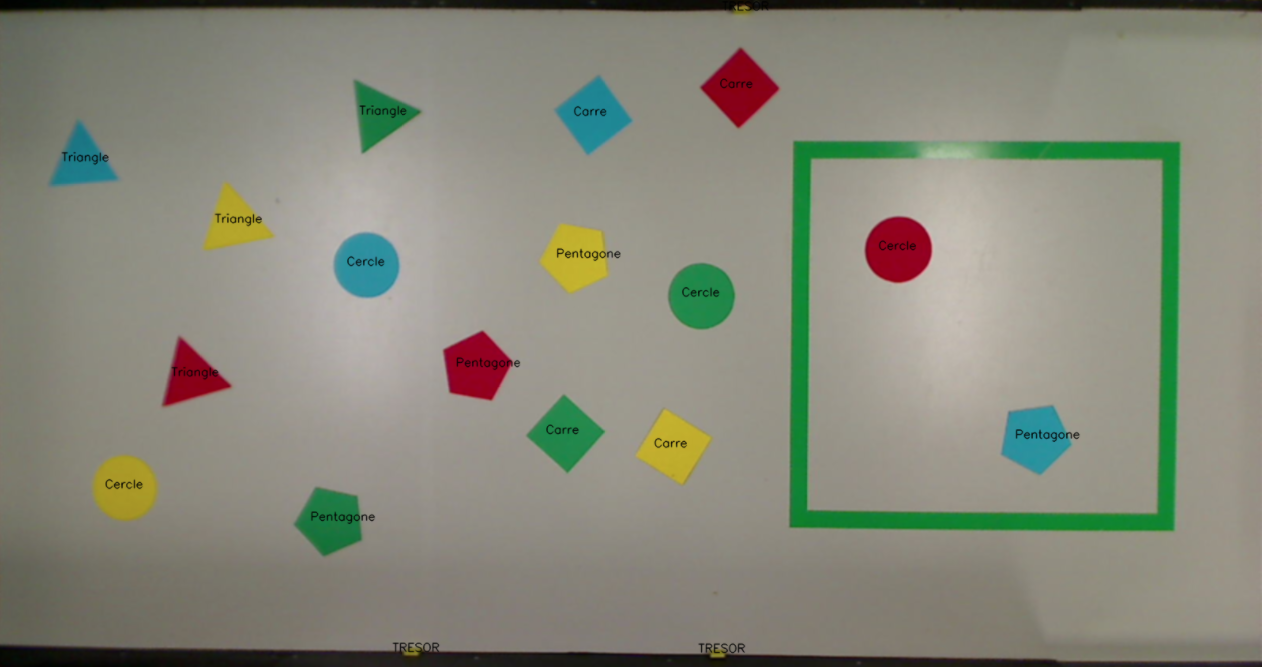
\includegraphics[width=1\textwidth]{fig/DetectionForme.png}
   \caption{R�sultat de la d�tection des formes}
   \label{f:DetectionForme}
\end{figure}

Cette m�thode est beaucoup plus fiable que celle utilis�e au d�part. La m�thode initiale �tait de d�tecter le nombre de sommets des formes d�tect�es pour ensuite d�duire quelle forme il s'agissait. Cette m�thode avait une faiblesse particuli�rement pour les formes qui se ressemblent, comme le cercle et le pentagone. Cependant, avec notre nouvelle m�thode, les taux de compatibilit�s sont tr�s pr�cis. En observant la figure \ref{f:PrecisionDetection}, une �le ronde poss�de un taux de compatibilit� d'environ 100 fois plus �lev� � un cercle qu'� un pentagone.

\begin{figure}[htp]
   \centering
   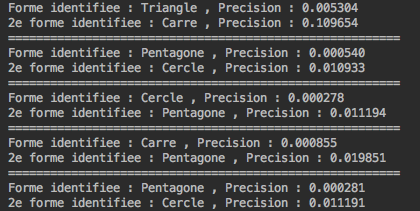
\includegraphics[width=0.7\textwidth]{fig/PrecisionDetection.png}
   \caption{Pr�cision de la d�tection des formes}
   \label{f:PrecisionDetection}
\end{figure}

\medbreak
Pour ce qui est du suivi de la position et de l'orientation du robot, un patron unique sera plac� au dessus de celui-ci afin d'avoir une r�f�rence facilement d�tectable. Le robot est le seul �l�ment que le syst�me de vision continue de d�tecter tout au long de la routine puisqu'il est le seul �l�ment mobile sur la carte de jeu.



%Les responsabilit�s du syst�me de vision sont partag�es entre la station de base et le robot. Le syst�me de vision sert � faire une analyse en profondeur de la table de jeu et � prendre des d�cisions gr�ce aux informations venant du robot. Le syst�me doit donc �tre performant et stable afin de ne pas induire le robot en erreur. 
\medbreak
La station de base, par l'entremise de la cam�ra monde, g�re la phase de d�placement tandis que le robot g�re la phase d'alignement � l'aide de sa cam�ra embarqu�e. La phase de d�placement comporte la d�tection des �l�ments cartographiques ainsi que la planification de la trajectoire alors que la phase d'alignement permet au robot de se positionner de mani�re optimale afin de faciliter l'ex�cution de la t�che demand�e.
\medbreak
La cam�ra monde est utilis�e pour la d�tection des �l�ments cartographiques ainsi que pour suivre le d�placement du tr�sor. Gr�ce � ces informations, la station de base peut g�n�rer une trajectoire et transmettre des commandes au robot.
\medbreak
La cam�ra embarqu�e ne sera utilis�e que dans deux situations. Tout d'abord, elle servira lorsque aucun tr�sor n'est d�tect� par la cam�ra monde, le robot tentera alors d'identifier la position des tr�sors gr�ce � son point de vue plus rapproch�. Ensuite, elle sera utilis�e lors de la phase d'alignement, afin que le robot puisse se rapprocher s�curitairement d'une cible comme une �le, un tr�sor ou la station de recharge. Donc, une fois la phase de d�placement termin�e et le robot rendu devant la cible, le syst�me de vision du robot prendra le contr�le afin d'amorcer la phase d'alignement.  



%!TEX encoding = IsoLatin

%
% Chapitre "Introduction"
%

%Sites d'achats, factures, etc


\begin{thebibliographyUL}{99} % remplacer le "{9}" par "{99}" lorsque le nombre de references
                              % requiert 2 caracteres (>= 10 references)
\bibitem{MOD00} Design II (mod�lisation), \textit{Actionneur �lectromagn�tique Partie 2}, [En ligne], \url{http://wcours.gel.ulaval.ca/2015/h/GEL2007/default/5notes/Seminaire_Actionneur_Balance_2015_part2fin.pdf}, Page consult�e le 17 f�vrier 2015

\end{thebibliographyUL}

\appendix
%%!TEX encoding = IsoLatin

%
% Annexe "Liste des sigles et des acronymes"
%

\chapter{Liste des sigles et des acronymes}
\label{Sigles}

\begin{flushleft}
   \begin{tabular}{@{}ll}
      \textbf{CAO}        & Conception Assist�e par Ordinateur \\
   \end{tabular}
\end{flushleft}



\end{document}          
